% ES 1402 Final Report (individual). Yellow brackets are placeholders to fill in.
% Needs device.jpg, five_notes.jpeg, plot_hw2.png, plot_hw3.png in the same folder.

\documentclass[11pt]{article}

\usepackage[utf8]{inputenc}
\usepackage[T1]{fontenc}
\usepackage{geometry}
\geometry{letterpaper, margin=1in}
\usepackage{amsmath}
\usepackage{amssymb}
\usepackage{graphicx}
\usepackage{float}
\usepackage{xcolor}
\usepackage{soul}
\usepackage{booktabs}
\usepackage{array}
\usepackage{setspace}
\usepackage{fancyhdr}
\usepackage[labelfont=bf,font=small]{caption}
\usepackage{hyperref}
\hypersetup{colorlinks=true, urlcolor=blue, pdfborder={0 0 0}}

\setstretch{1.08}
\setlength{\parskip}{0.5em}
\setlength{\parindent}{0pt}
\sethlcolor{yellow}
\newcommand{\ph}[1]{\hl{[#1]}}

\pagestyle{fancy}
\fancyhf{}
\fancyfoot[C]{\thepage}
\renewcommand{\headrulewidth}{0pt}

\begin{document}

%% ------------------------- Title page -------------------------
\thispagestyle{empty}
\begin{center}
    \vspace*{1.5cm}

    {\LARGE\bfseries Team primitive}\\[2.5cm]
    {\fontsize{40}{48}\selectfont\bfseries Final Report}\\[0.8cm]
    {\Large Hot Cross Buns}\\[2.5cm]
    {\large
    Hudson Mills\\
    Kyuri Lim\\
    \textbf{Youssef Nassar}\\
    G\"um\"u\c{s}su Memik}\\[2.5cm]
    {\large ES 1402-13, Introduction to Engineering Module 2\\
    Vanderbilt University, Fall 2026\\
    November 3}
\end{center}
\newpage

%% ------------------------- 1 Introduction -------------------------
\section{Introduction}

Our team built four instruments tuned to the same piano notes. I built a set of five water-bottle Helmholtz resonators. G\"um\"u\c{s}su built closed-end straw flutes (A4 to G4, tuned by length), Kyuri built open-end straw flutes (E5 to B5), and Hudson built a full-range gamelan of 52 stainless steel bars (A3 to C8). On a personal level, my objective was to learn fundamentals of acoustics and challenge my interests which are predominantly in digital electronics.

%% ------------------------- 2 Design and Construction -------------------------
\section{Design and Construction}

Each note comes from one Helmholtz resonator, a closed bottle with a narrow neck, which rings at
\begin{equation}
f = \frac{c}{2\pi}\sqrt{\frac{A}{V\,L_\mathrm{eff}}} ,
\end{equation}
where $c = 331.3 + 0.606\,T = 343.4$ m/s at 20\,$^\circ$C, $A$ is the neck area, $V$ is the air volume, and $L_\mathrm{eff} = L + 0.85\,d$. Only $V$ was changed, so $f \propto V^{-1/2}$.

\begin{center}
\renewcommand{\arraystretch}{1.3}
\begin{tabular}{@{}>{\raggedright}p{1.1in}p{5.2in}@{}}
\toprule
Component & Details \\
\midrule
Bottle & 355 mL Aquafina PET bottle, brim volume 393 mL \\
Neck & $d = 21.78$ mm, $L = 23.89$ mm, $A = 3.73\times10^{-4}$ m$^2$, $L_\mathrm{eff} = 42.4$ mm \\
Tuning & Water level. Each bottle started with 343 mL of water (50 mL of air), and water was removed with a 60 mL syringe \\
Tools & 60 mL syringe, Friture, MATLAB; room temperature 20\,$^\circ$C \\
\bottomrule
\end{tabular}
\end{center}

The first design changed the air volume with a 60 mL syringe plunger taped to the bottle (Figure~\ref{fig:device}). The thin walls caved in when the plunger was pulled, so the air volume and the pitch barely changed. Tuning was switched to water level. The final instrument has five identical bottles for D4, E4, F4, G4, and C5 (Figure~\ref{fig:five}).

\begin{figure}[H]
\centering
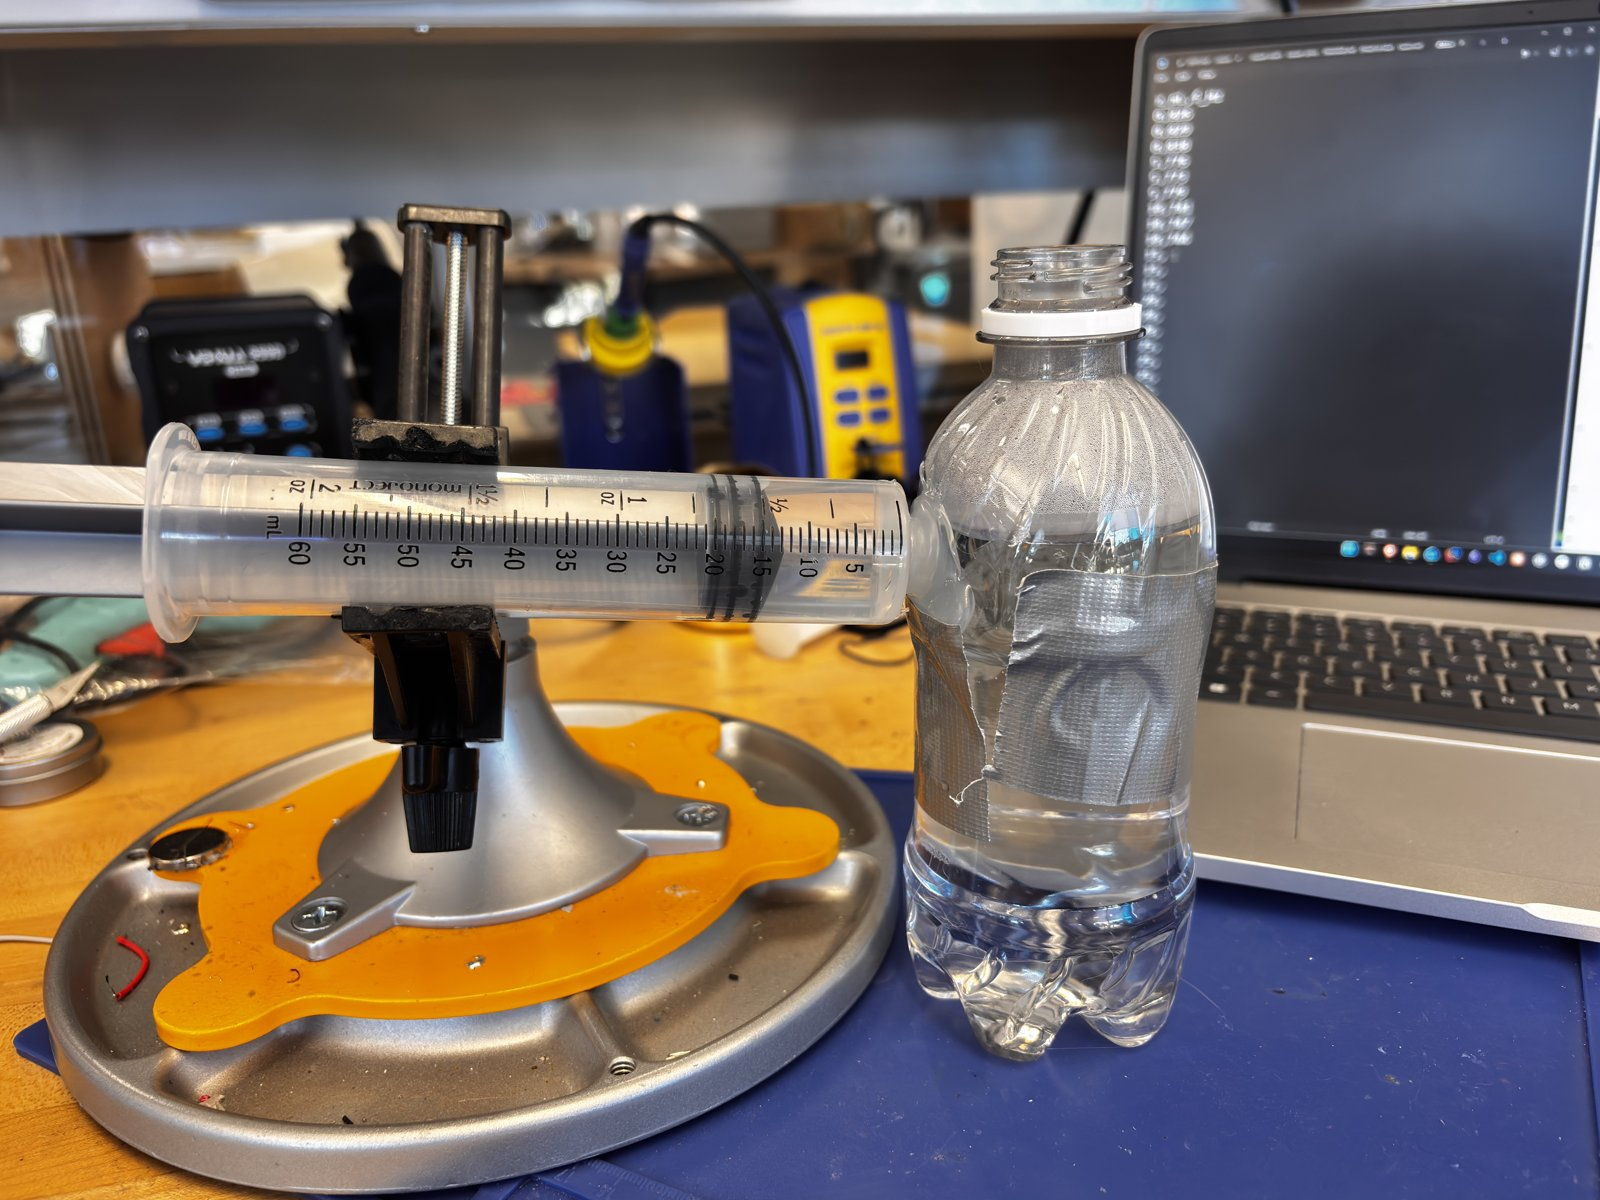
\includegraphics[width=0.52\linewidth]{device.jpg}
\caption{First design: a 60 mL syringe attached to the side of the bottle.}
\label{fig:device}
\end{figure}

\begin{figure}[H]
\centering
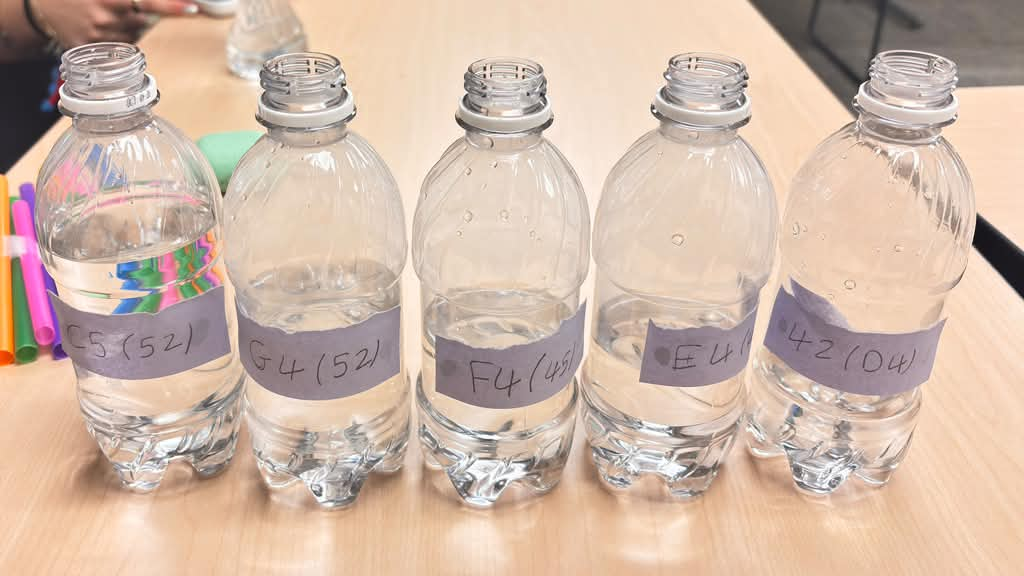
\includegraphics[width=0.8\linewidth]{five_notes.jpeg}
\caption{The final instrument: C5, G4, F4, E4, and D4 from left to right.}
\label{fig:five}
\end{figure}


%% ------------------------- 3 Testing Results -------------------------
\section{Testing Results}

\subsection{Single-note tuning test (HW 2)}

One bottle started with 50 mL of air. Water was removed in 5 mL steps ($x = 0$ to 30 mL), and Friture was read three times per step. The model $f = a/\sqrt{V_0 + x}$ was linearized as
\begin{equation}
\frac{1}{f^{2}} = \frac{1}{a^{2}}\,x + \frac{V_0}{a^{2}}
\end{equation}
and fitted with \texttt{polyfit}, giving $a = 1/\sqrt{\text{slope}}$ and $V_0 = \text{intercept}/\text{slope}$ (Figure~\ref{fig:hw2}).

\begin{center}
\small
\renewcommand{\arraystretch}{1.2}
\begin{tabular}{lccccccc}
\toprule
$x$ (mL) & 0 & 5 & 10 & 15 & 20 & 25 & 30 \\
\midrule
Mean $f$ (Hz) & 831.0 & 776.0 & 744.0 & 710.0 & 682.0 & 627.0 & 588.0 \\
SD (Hz) & 6.2 & 3.0 & 3.0 & 1.7 & 3.5 & 3.0 & 1.7 \\
\bottomrule
\end{tabular}
\end{center}

\begin{figure}[H]
\centering
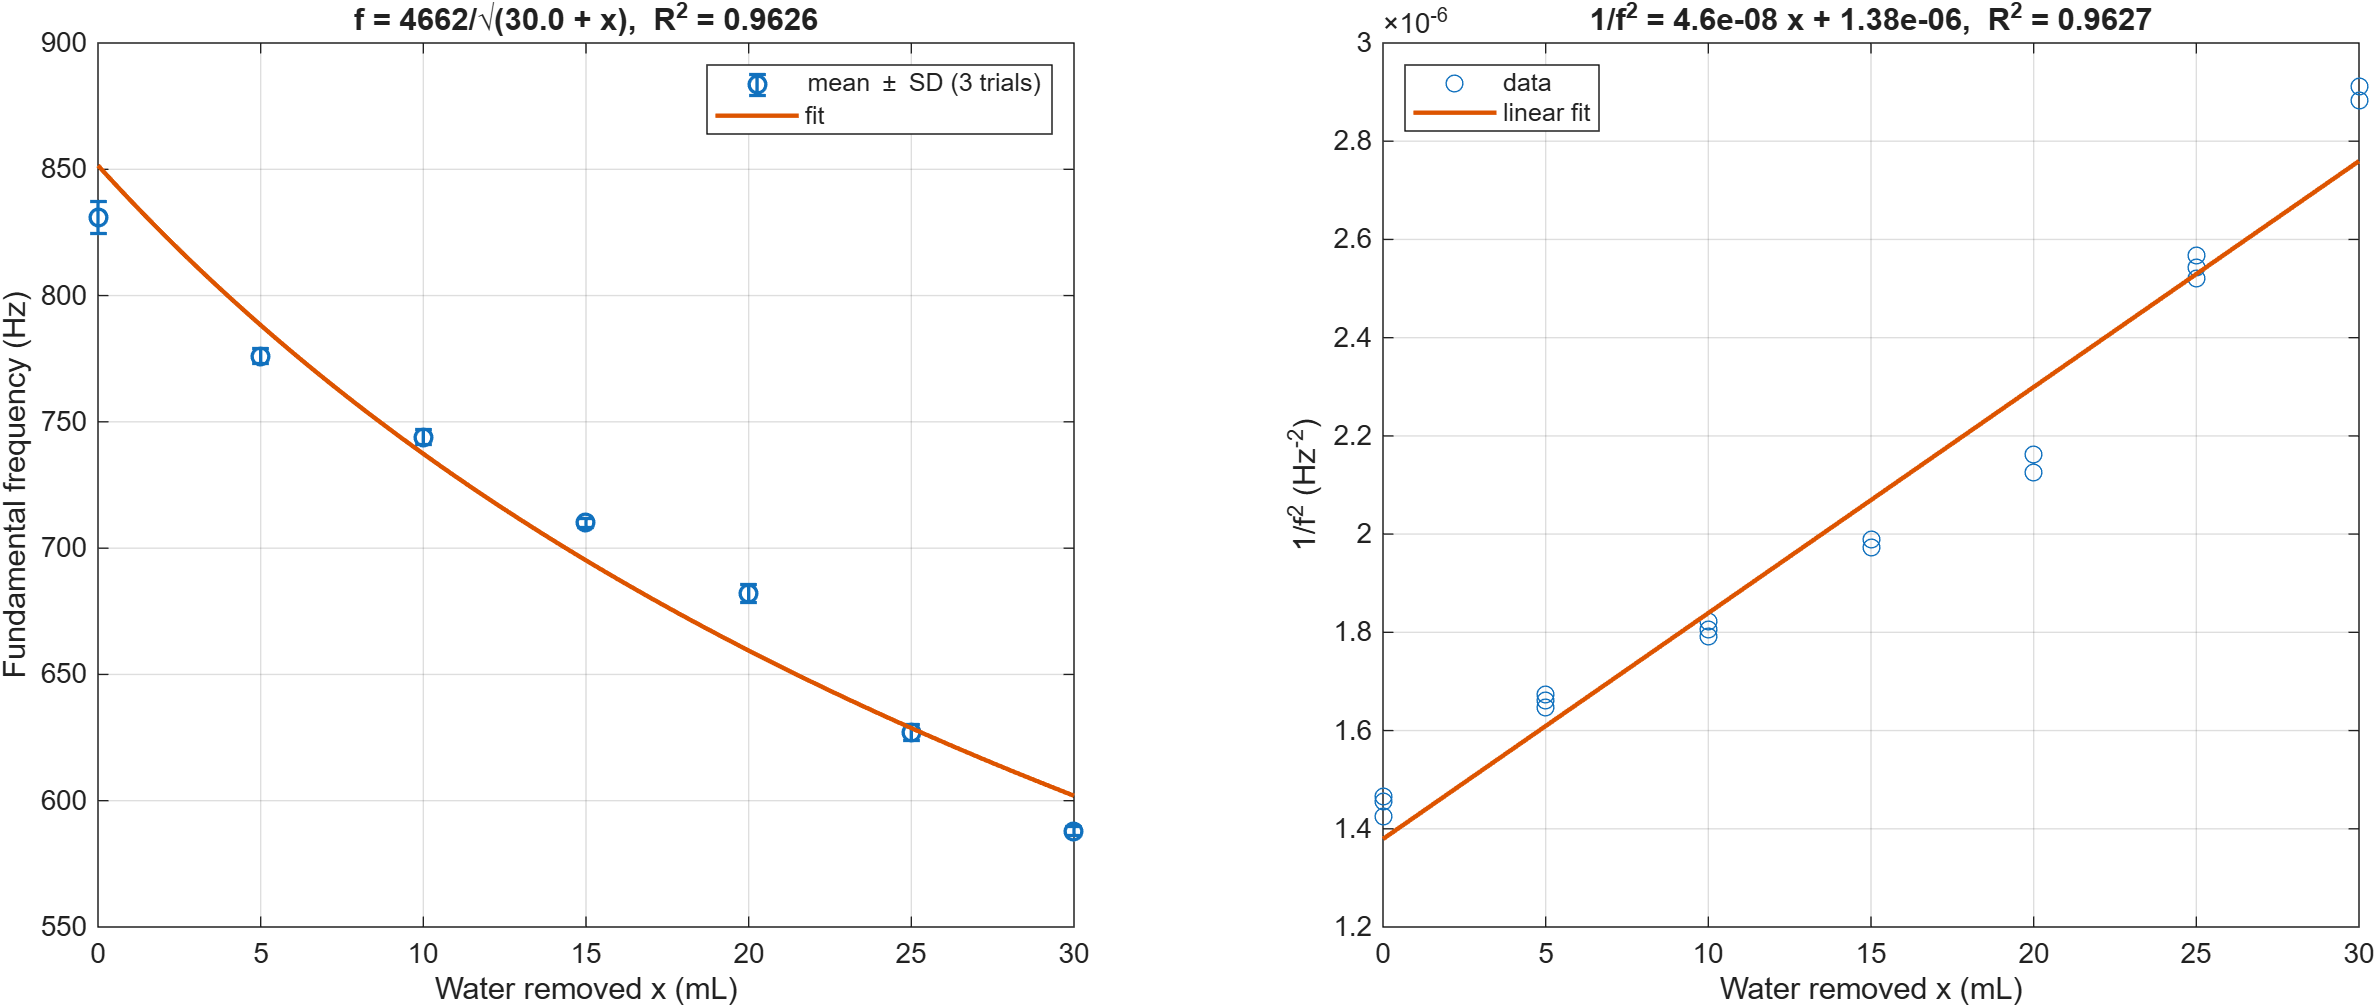
\includegraphics[width=\linewidth]{plot_hw2.png}
\caption{Left: frequency against water removed (mean $\pm$ SD) with the fit. Right: $1/f^2$ against $x$.}
\label{fig:hw2}
\end{figure}

With all seven points, $a = 4662$ (theory 5123), $V_0 = 30.0$ mL (expected about 41 mL), and $R^2 = 0.963$. The last two steps changed $1/f^2$ about twice as much as the earlier ones, and the cause was not confirmed. With $x \le 20$ mL, $a = 5381$, $V_0 = 42.4$ mL, and $R^2 = 0.994$, which agrees with theory. A 2\% change in air volume changed the pitch by about 1\%, so water had to be changed in small steps.

\subsection{Five-note instrument (HW 3)}

Each bottle was tuned until the main Friture peak matched its target, and three readings were taken. Piano notes follow $f = 440\cdot2^{(n-49)/12} = A\,e^{kn}$ with $A = 25.96$ Hz and $k = \ln 2/12 = 0.05776$. Taking $\ln f$ gives a straight line in $n$, which was fitted with \texttt{polyfit} (Figure~\ref{fig:hw3}).

\begin{center}
\small
\renewcommand{\arraystretch}{1.2}
\begin{tabular}{cccccc}
\toprule
Note & Key $n$ & Target (Hz) & Mean (Hz) & SD (Hz) & Difference \\
\midrule
D4 & 42 & 293.7 & 291.0 & 1.7 & $-0.9\%$ \\
E4 & 44 & 329.6 & 327.3 & 1.2 & $-0.7\%$ \\
F4 & 45 & 349.2 & 349.0 & 1.0 & $-0.1\%$ \\
G4 & 47 & 392.0 & 392.0 & 1.7 & $0.0\%$ \\
C5 & 52 & 523.3 & 521.3 & 2.5 & $-0.4\%$ \\
\bottomrule
\end{tabular}
\end{center}

\begin{figure}[H]
\centering
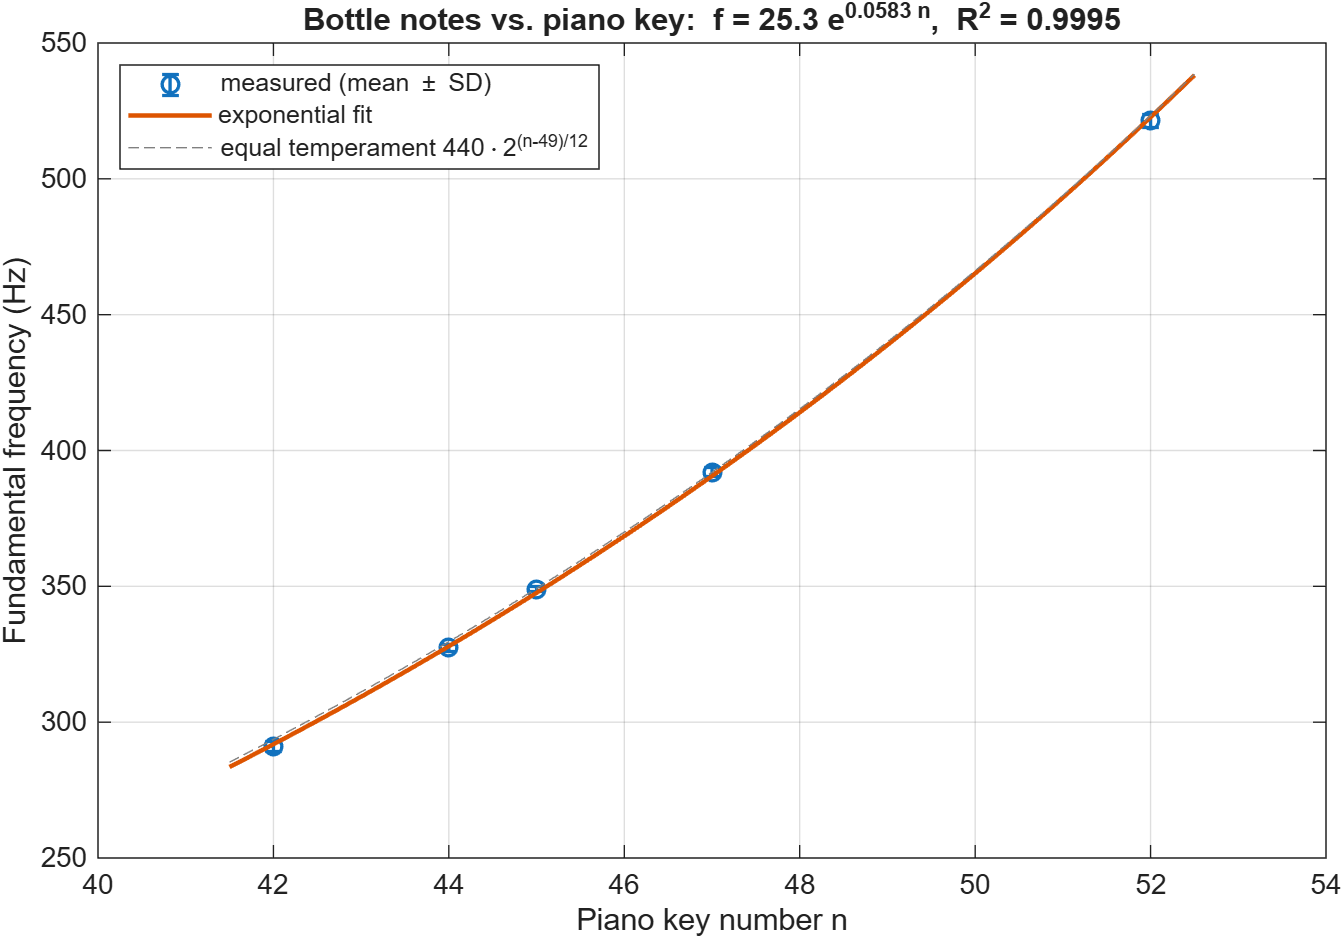
\includegraphics[width=0.78\linewidth]{plot_hw3.png}
\caption{Measured frequency against key number (mean $\pm$ SD), the exponential fit (solid), and equal temperament (dashed).}
\label{fig:hw3}
\end{figure}

The fit gave $f = 25.3\,e^{0.0583\,n}$ with $R^2 = 0.9995$. The fitted $k$ is 0.9\% above theory, and the fitted A4 is 439 Hz against 440 Hz. With five notes tuned to the scale, a high $R^2$ is expected, so the per-note differences matter more.

%% ------------------------- 4 Final Results -------------------------
\section{Final Results and Discussion}

\subsection{Individual performance}

Every note is within 1\% of its piano frequency, and repeated readings agreed within 1 to 3 Hz. D4 and E4 are slightly flat. The instrument was used to play ``Hot Cross Buns''. Only three notes were used, so the flatness of D4 and E4 was not noticeable. My instruments was the quietest of the four, and the high notes were hard to hear.

\subsection{Power spectrum and timbre}

Each note was identified from the tallest peak in the Friture spectrum, which is the resonance of the bottle (Section 3.2). The peaks were wide and noisy because of the breath, and the three readings of each note differed by an SD of 1.0 to 2.5 Hz, or 0.3\% to 0.6\% of the frequency. G4 was the hardest to read, with a second peak close to 400 Hz. A bottle has one resonance, so the tone is close to a single frequency and sounds soft, while the gamelan bars have overtones and sound brighter.

\subsection{Team performance}

The presentation and teamwork was smooth as everything was communicated before hand, except that one of the teammembers was absent as they did not communicate that before the final presentation. However the recording and building the presentation slides were straighforward.
\subsection{Improvements and critical limitations}

Tuning resolution was the main limit. A few millilitres of water decide the note, so the water level should be set with a burette or a scale. Two improvements are planned:
\begin{itemize}
\item Make one 3D-printed bottle with a spring-loaded syringe, so its air volume can be controlled and the note switched easily without five separate bottles. A rigid wall would also avoid the caving seen in the first design.
\item Build a simple trumpet as a further instrument.
\end{itemize}
Other limits were the quiet high notes (little air) and the flexing of the thin plastic walls, which acts as extra volume.

%% ------------------------- 5 Feedback -------------------------
\section{Feedback}

\subsection{What I learned and enjoyed}

I learned the physics behind musical instruments, and got more familiar with MATLAB. I enjoyed seeing the same piano notes made with different physics: a bottle, a closed tube, an open tube, and steel bars.

\subsection{How the project and course could be improved}

I honestly have no comments; I think the course was quite fun and interesting (I might argue that the little tangents were equally if not more insightful as the course content!)

\end{document}
